\documentclass[journal]{IEEEtran}
\usepackage{cite}
\usepackage{amssymb}
\usepackage{amsmath}
\usepackage{graphicx}

\graphicspath{ {figures/} }

\title{Optimizing Compressed Sensing Sensing Matrices}
\author{Nicholas McKibben and Connor Anderson}

\begin{document}
\maketitle
\thispagestyle{empty}
\pagestyle{empty}
%%%%%%%%%%%%%%%%%%%%%%%%%%%%%%%%%%%%%%%%%%%%%%%%%%%%%%%%%%%%%%%%%%%%%%%%%%%%%%%%
\begin{abstract}

Compressed Sensing (CS) is a technique for reconstructing a signal that has been sampled well below the Nyquist-Shannon criterion.  In general, it is impossible to recover an undersampled signal: there is no way to know what the missing information was. However, when the original signal meets certain constraints, it becomes possible to recover it from its undersampled representation with a high (or even perfect) degree of accuracy. Compressed sensing is a method for recovering signals that have been highly undersampled that meet two constraints. First, it must have a sparse representation in some transform domain. Second, the sampling must be accomplished in such a way so that the resulting aliasing is incoherent. Luckily, many signals of interest can be shown to have sparse representations is some domain, such as the Wavelet Transform or the Discrete Cosine Transform. If those signals are then sampled in the right way, they can be represented by far fewer data points but recovered almost exactly.  This project demonstrates an algorithm that optimizes the sensing matrix for basis pursuit CS reconstruction.

\end{abstract}
%%%%%%%%%%%%%%%%%%%%%%%%%%%%%%%%%%%%%%%%%%%%%%%%%%%%%%%%%%%%%%%%%%%%%%%%%%%%%%%%

%%%%%%%%%%%%%%%%%%%%%%%%%%%%%%%%%%%%%%%%%%%%%%%%%%%%%%%%%%%%%%%%%%%%%%%%%%%%%%%%
\section{INTRODUCTION}

The notion of sparse representation and reconstruction is actually a well-studied problem within statistics, first described by Santosa and Symes in 1986 \cite{santosa}.  But the ramifications of the robustness of the reconstructions provided by this theory have only started to be realized in the past decade, with an emphasis on sparse sensing instead of retroactive application to already complete datasets, hence the name ``compressed sensing'' \cite{donoho}.

This reemergence of CS grew out of the pioneering work of Cand\`es, Romberg, Tao, and Donoho, who demonstrated that \emph{n}-dimensional signals with sparse representations can be exactly reconstructed from a set of linear, non-adaptive measurements in a wide variety of cases \cite{csbook,baraniuk,candes,donoho}.

CS differs from classical sampling theory in a few important ways.  First, classical sampling theory typically considers infinite dimensional, continuous-time signals.  CS restricts itself to finite, \emph{n}-dimensional signals.  Secondly, CS formulations usually do not sample the signal at specific points in time as is done classically.  Rather, measurements are acquired in the form of inner products between the signal and more general test functions (usually including some random component) \cite{csbook}.  Lastly, Nyquist-Shannon relies on sinc interpolation, whereas CS signal recovery typically uses highly non-linear methods \cite{oppenheimdigital,csbook}.

Successful CS reconstruction is achieved if certain properties of the sampling operator, or sensing matrix, can be guaranteed (e.g., the Restricted Isometry Property, mutual coherence minimization, or the nullspace property \cite{tcs}).  These properties ensure sufficient conditions on the equivalent sensing matrix\footnote{The equivalent sensing matrix is the product of the sensing matrix and the sparsifying basis} for accurate signal recovery. Random matrices (i.e., Gaussian or Bernoulli) are known to satisfy these properties for any given sparsifying basis and are used widely sensing matrices in many CS applications.

In 2007, Michael Elad demonstrated that minimizing the mutual coherence of a projection matrix $P$ (the sampling operator) improves CS reconstruction \cite{elad}.  In this paper we will present the main theory behind the optimization, the results of our implementation, and a discussion of the merits and pitfalls of Elad's algorithm.

\section{MATH}

Here we describe the math behind our CS implementation.  For a set of signals $\{x_j \in \mathbb{R}^n\}$ that we are interested in measuring, we assume that each $x_j$ has a sparse representation in some transform domain, such as the Discrete Cosine Transform (DCT).  If we have a dictionary of vectors $D \in \mathbb{R}^{n\times k}$ whose columns span the transform domain, then we represent $x_j$ as a linear combination: $x_j = D\alpha_j$, where $||\alpha_j||_0 \ll n$, with the $\ell_0$-norm describing $\alpha$ as a sparse vector.  If this is the case, then our signal $x_j$ can be accurately (or perfectly) represented in a much-lower dimensional vector space $\mathbb{R}^p$ as $$y_j = Px_j=PD\alpha_j$$ where $P \in \mathbb{R}^{p\times n}$ with $p \ll n$ is the projection matrix from $\mathbb{R}^n$ to the lower-dimensional space $\mathbb{R}^p$.  We can then recover each $x_j$ from $y_j$ by finding the sparsest $\alpha$ that satisfies $y_j = PD\alpha_j$.

We now have a projection matrix to solve the CS problem: $$ \min_\alpha ||\alpha||_0 \mbox{ subject to } y = Px = PD\alpha.$$  The $\ell_0$ quasi-norm is known to be NP-hard and is shown to be approximately equivalent in most cases to the more tractable convex optimization problem using the $\ell_1$ norm \cite{convexoptimization}, so we solve the so-called Basis Pursuit (BP) linear program: $$ \min_\alpha ||\alpha||_1 \mbox{ subject to } y = PD\alpha .$$

For a given dictionary $D$, its mutual coherence, $\mu$, is the largest absolute inner product between its columns and represents the worst similarity between dictionary columns.  This similarity is problematic for BP solvers, and we would like to minimize it to improve reconstructions.  Mathematically we show mutual coherence for  as: $$ \mu\{D\} = \max_{i \leq i,j \leq k, i \neq j} \frac{| d_i^Td_j |}{|| d_i || \cdot || d_j ||}. $$

Elad points out that we can find the same quantity by considering $D$'s gramian, $G = \hat{D}^T \hat{D}$, where $\hat{D}$ is $D$ with normalized columns.  The largest off-diagonal entry of $G$ is $\mu\{D\}$ as it is defined above.  Now, the effective dictionary is $PD$, and we must optimize $\mu\{PD\}$ with respect to $P$.  It turns out that when we consider the average performance of a wider class of signals, the mutual coherence provides a poor optimization and such a method is likely to be far more complex.  With this in mind, Elad suggests that the average measure of coherence is more likely to describe the true behavior using the modified $t$-averaged mutual coherence: $$ \mu_t\{PD\} = \frac{ \sum_{1 \leq i,j \leq k, i \neq j} (| g_{ij} | \geq t) \cdot | g_{ij} | }{ \sum_{1 \leq i,j \leq k, i \neq k} (\ | g_{ij} | \geq t)} $$ where $g_{ij}$ are entries of the $PD$'s Gram matrix with normalized columns.

From this $t$-averaged metric, we can see that our main objective is the reduction of the inner products that are above some known threshold $t$.  We achieve this by shrinking the entries of the Gram matrix by a factor $\gamma$ while preserving the entries' ordering.  The ``shrunken'' Gram matrix is then decomposed into a squared-root matrix $G = S^TS$ which is used to solve for the new projection matrix $P$ by finding the $P$ that minimizes $ || S - PD ||_F^2 $.

\section{RESULTS}

We were able to successfully implement the algorithm as presented in the paper and observe the similar results to those presented.  As our implementation did not use some of the BP optimizations that the paper used, it ran an order of magnitude more slowly and we reduced matrix sizes and signal averages in order to run the experiments in a reasonable time.

To show the behavior of our implementation, we constructed a random dictionary $D \in \mathbb{R}^{200 \times 400} $ with each entry drawn from an i.i.d. zero mean, unit variance Gaussian distribution with initial projection matrix $P$ formed the same way in $\mathbb{R}^{30 \times 200}$.  After $50$ iterations and with appropriate choice of $t$ and $\gamma$, our algorithm produced a converging plot of $\mu_t\{PD\}$ as shown in Figure \ref{fig:mu_t}.  With more signal averages $x_j$, we anticipate that this curve would smooth even more.

\begin{figure}[]
  \centering
  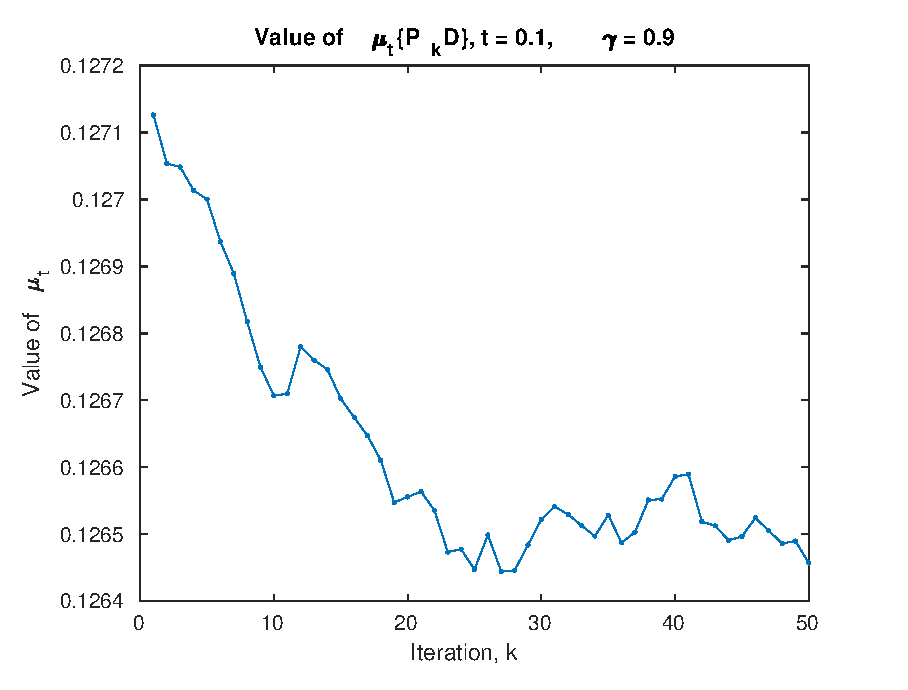
\includegraphics[width=0.45\textwidth]{mu_t.eps}
  \caption{Value of $\mu_t\{P_kD\}$ as a function of the iteration for $t = 0.1$ and $\gamma = 0.9$.  As $k$ increases, $\mu_t$ converges to the value of $t$.}
  \label{fig:mu_t}
\end{figure}

Constructing a smaller $150 \times 250$ redundant DCT dictionary with $p$ varying from $21$--$25$ we found that optimizing $P$ with $200$ iterations and $15$ averaged test signals $x_j$ did make a difference and improved the reconstruction compared to only random choices of $P$.  Figure \ref{fig:err} shows the CS errors as a function of $p$.  Although the difference between the error is small in our experiment, we observed that increasing the number of iterations, number of signal averages, and matrix dimensions, while computationally expensive especially using our numerical code, increases the error gap and provides more faithful reconstructions.

\begin{figure}[]
  \centering
  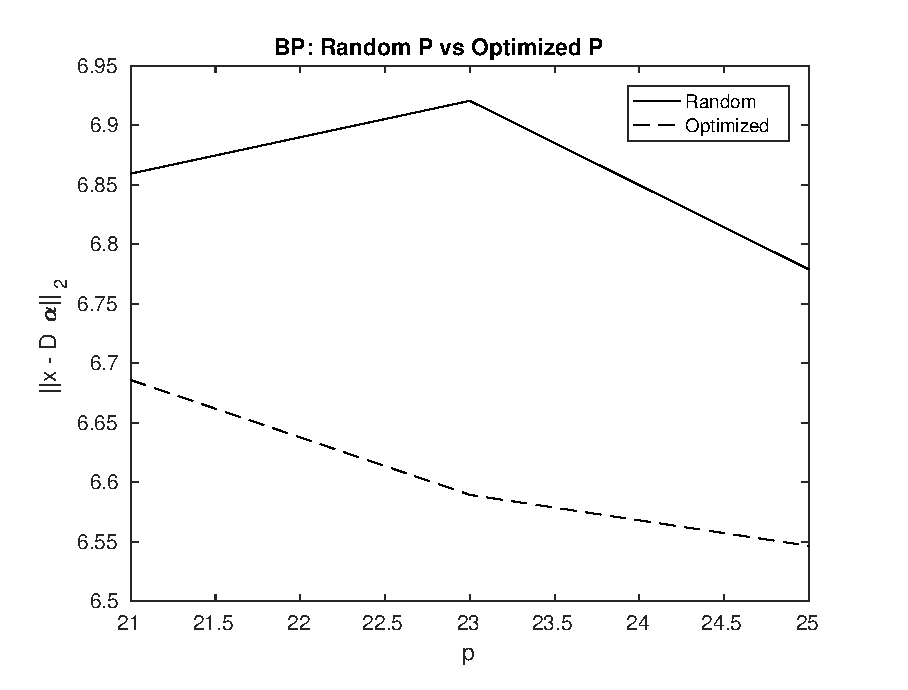
\includegraphics[width=0.45\textwidth]{rel_errors.eps}
  \caption{CS errors as a function of the number of measurements $p$ with randomly generated $P$ and optimized projections $P_{opt}$.}
  \label{fig:err}
\end{figure}

To visualize the change in the projection matrix $P$ after optimization, we recreated a histogram showing the absolute off-diagonal entries of the Gram matrix $G$ before and after the algorithm was run using 

\begin{figure}[]
  \centering
  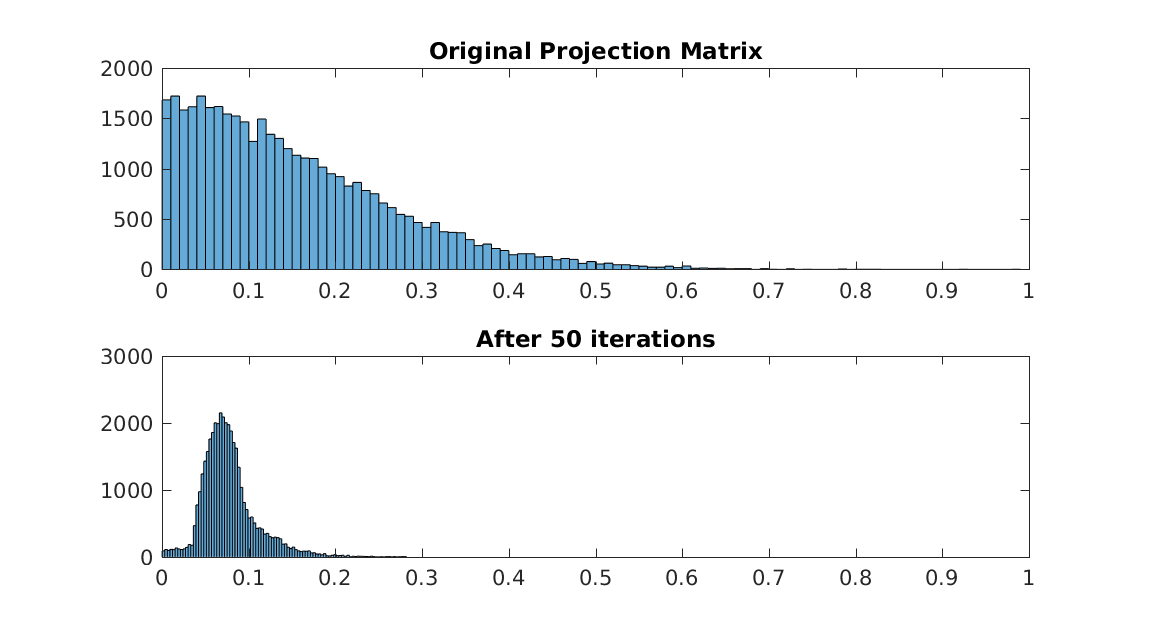
\includegraphics[width=0.45\textwidth]{hist.eps}
  \caption{CS errors as a function of the number of measurements $p$ with randomly generated $P$ and optimized projections $P_{opt}$.}
  \label{fig:hist}
\end{figure}

%%%%%%%%%%%%%%%%%%%%%%%%%%%%%%%%%%%%%%%%%%%%%%%%%%%%%%%%%%%%%%%%%%%%%%%%%%%%%%%%
\section{DISCUSSION}




%%%%%%%%%%%%%%%%%%%%%%%%%%%%%%%%%%%%%%%%%%%%%%%%%%%%%%%%%%%%%%%%%%%%%%%%%%%%%%%%
\bibliographystyle{IEEEtran}
\bibliography{project}{}
%%%%%%%%%%%%%%%%%%%%%%%%%%%%%%%%%%%%%%%%%%%%%%%%%%%%%%%%%%%%%%%%%%%%%%%%%%%%%%%%

\end{document}
